\documentclass[10pt]{beamer}

\usepackage{fontspec}
\usepackage{xunicode}
\usepackage{xltxtra}
\setsansfont{FreeSans}
\setmonofont{DejaVuSansMono}

\usepackage{listings}
\usepackage{textpos}
\usepackage{tikz}
\usepackage{minted}

\setbeamertemplate{footline}[frame]
\setbeamertemplate{items}[default]
\usetheme{Warsaw}
\usecolortheme{seahorse}
\setbeamertemplate{itemize items}[default]
\setbeamertemplate{navigation symbols}{}
\setbeamertemplate{footline}[frame number]
\lstset{columns=fixed}
\setbeamerfont*{block body}{series=\tt}
\definecolor{lightgray}{rgb}{0.95,0.95,0.95}
\definecolor{midgray}{rgb}{0.5,0.5,0.5}

\newcommand{\light}[1]{\textcolor{gray}{\footnotesize{#1}}}
\newcommand{\code}[4]{\inputminted[linenos, frame=none, firstline=#2, lastline=#3,
  framesep=10pt, bgcolor=lightgray]{#4}{#1}}

\title[Об ошибках]{Обработка ошибок — общие соображения и грязные подробности}
\author{Дмитрий Грошев}
\date{
\includegraphics[height=3cm]{add-large}\\11.05.2012}
\institute{}

\addtobeamertemplate{frametitle}{}{%
\begin{textblock*}{100mm}(1\textwidth,-0.7cm)

\includegraphics[height=0.6cm]{add.png}
\end{textblock*}}

\begin{document}

\begin{frame}
\titlepage
\end{frame}

\begin{frame}{}
  \begin{center}
    \huge Вступление
  \end{center}
\end{frame}

\begin{frame}{Ошибки}
  \begin{center}
    Все делают ошибки, однако некоторые думают об ошибках так:\vspace{3mm}\\
    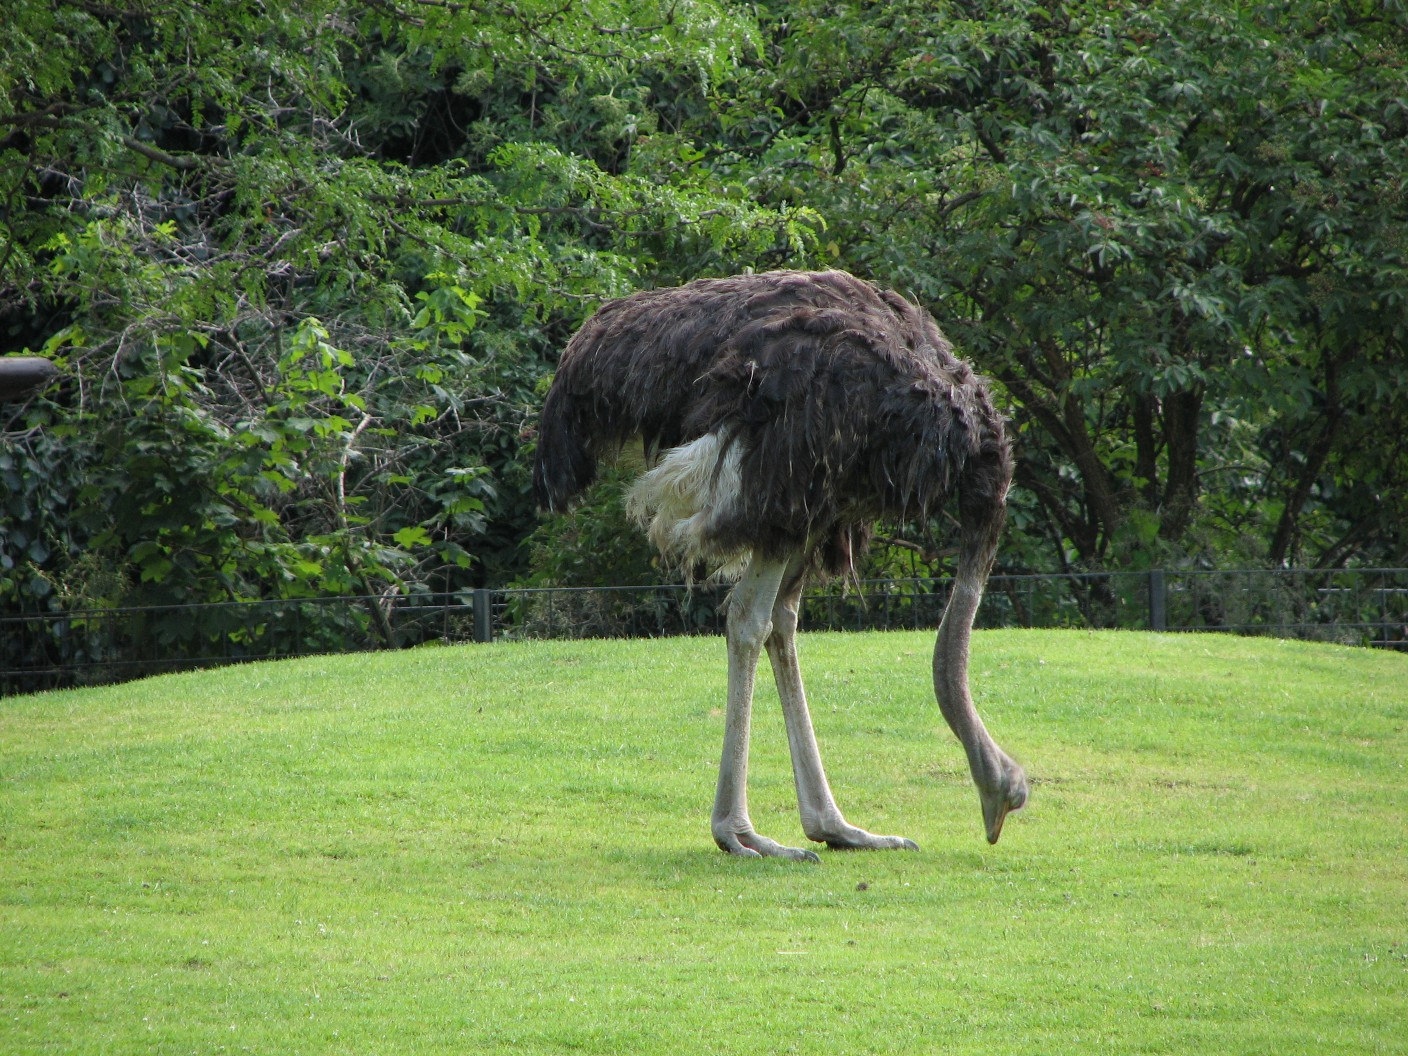
\includegraphics[height=6cm]{ostrich}
  \end{center}
\end{frame}

\begin{frame}{Ошибки}
  \begin{center}
    Но лучше делать это так:\vspace{3mm}\\
    
\includegraphics[height=6cm]{attack}
  \end{center}
\end{frame}

\begin{frame}{Ошибки}
  \begin{center}
    Для этого нужно знать о враге больше!
  \end{center}
\end{frame}

\begin{frame}{Короткий план доклада}
  \begin{itemize}
  \item общие соображения
    \begin{itemize}
    \item классификация ошибок
    \item о балансе
    \item простые и сложные ошибки
    \item третий путь
    \item всё ещё хуже — ошибки перегрузки, ошибки параллелизма
    \end{itemize}
  \item грязные подробности
    \begin{itemize}
    \item исторически сложившиеся методы обработки ошибок
    \item снова о статике и немного о монадах
    \item велосипеды
    \item пример кода
    \end{itemize}
  \end{itemize}
\end{frame}

\begin{frame}{}
  \begin{center}
    \huge Часть 1: общие соображения
  \end{center}
\end{frame}

\begin{frame}{Классификация}
  Наиболее очевидная классификация:
  \begin{itemize}
  \item времени компиляции
  \item времени выполнения
  \end{itemize}
\end{frame}

\begin{frame}{Ремарка о балансе}
  Когда ловить ошибки?
  \begin{itemize}
  \item во время компиляции — код либо сложнее, либо многословнее
  \item во время выполнения — падает надёжность
  \end{itemize}
  Необходим баланс между этими крайностями
\end{frame}

\begin{frame}[fragile]{«Простые» ошибки}
  Ошибки бывают очевидными:
  \code{code.py}{1}{3}{python}
  \begin{itemize}
  \item JS: «это не ошибка»
  \item Python: «добавь try/except»
  \item Java: «где типы?»
  \end{itemize}
\end{frame}

\begin{frame}{«Это не ошибка»}
  \begin{center}
    \light{Этот слайд оставлен пустым в память всех жертв плохого дизайна}
  \end{center}
\end{frame}

\begin{frame}{«Добавь try/except»}
  \code{code.py}{5}{10}{python}
  \begin{itemize}
  \item повседневная реальность большинства разработчиков
  \item требует юнит-тестов
  \item 100\% покрытие ничего не гарантирует
  \end{itemize}
\end{frame}

\begin{frame}{«Где типы?»}
  \code{code.java}{1}{7}{java}
  \begin{itemize}
  \item этот код даже не скомпилируется
  \item этого кода слишком много
  \item люди не любят писать много и отказываются от типов вообще
  \end{itemize}
\end{frame}

\begin{frame}{«Где типы?»}
  \code{code.hs}{1}{3}{haskell}
  \begin{itemize}
  \item этот код тоже не скомпилируется
  \item типы a и b однозначно вытекают из соответствующих литералов — зачем их указывать?
  \item компилятор может пытаться выводить типы сам
  \item не все корректные программы могут пройти проверку типов
  \end{itemize}
\end{frame}

\begin{frame}{Проблема статической типизации}
  Ещё раз: \emph{не все корректные программы статически типизируемы}\vspace{2em}\\
  Или: \emph{любая система типов может мешать программисту}
\end{frame}

\begin{frame}{Проблема статической типизации}
  Пример:
  \code{code.java}{17}{23}{java}
\end{frame}

\begin{frame}{Оптимистичная типизация}
  \code{code.erl}{1}{4}{erlang}
  \begin{itemize}
  \item этот код скомпилируется
  \item тайпчекер (отдельная программа в случае Erlang'а) укажет на ошибку
  \end{itemize}
\end{frame}

\begin{frame}{Оптимистичная типизация}
  \code{code.erl}{6}{11}{erlang}
  \begin{itemize}
  \item тайпчекер не найдёт ошибки в этом коде
  \item «оптимистичная» = если тайпчекер не может вывести тип, считается, что всё хорошо
  \end{itemize}
\end{frame}

\begin{frame}{Оптимистичная типизация}
  Система типов:
  \begin{itemize}
  \item оптимистичная — пропускает часть ошибок (но все найденные ошибки существуют в реальности)
  \item пессимистичная — отклоняет часть корректных программ (но скомпилированная программа точно не содержит ошибок типов)
  \end{itemize}
\end{frame}

\begin{frame}{«Простые» ошибки: резюме}
  Проблема ошибок типов («простых» ошибок) более-менее решена
  \begin{itemize}
  \item статическая типизация с выводом типов
  \item оптимистичная типизация для динамических языков
  \end{itemize}
\end{frame}

\begin{frame}{«Сложные» ошибки}
  \code{code.java}{9}{15}{java}
  \begin{itemize}
  \item этот код скомпилируется
  \item где ошибка?
  \end{itemize}
\end{frame}

\begin{frame}{«Сложные» ошибки}
  \begin{itemize}
  \item в выражении [(a + b) / 2] a + b может быть больше, чем int
  \item это сложно увидеть глазами
  \item это не проверит компилятор
  \item 100\% coverage не поможет
  \item эти ошибки связаны со значениями (а не с типами)
  \end{itemize}
\end{frame}

\begin{frame}{Property-based тестирование}
  \code{code.erl}{13}{15}{erlang}
  \begin{itemize}
  \item тестирующая система сама может генерировать тесты
  \item предполагается, что в определении json нет ошибки
  \item вероятность найти «сложную» ошибку выше
  \end{itemize}
\end{frame}

\begin{frame}{Зависимые типы}
  \code{code.ats}{1}{3}{c}
  \begin{itemize}
  \item конкретные значения и их соотношения являются параметрами типов
  \item сложные компиляторы, очень сложно писать
  \end{itemize}
\end{frame}

\begin{frame}{«Сложные» ошибки: резюме}
  \begin{itemize}
  \item проблема не имеет общепринятого решения
  \item ошибки такого рода во время выполнения практически неизбежны
  \item что делать?
  \end{itemize}
\end{frame}

\begin{frame}{Good enough}
  Нужно:
  \begin{itemize}
  \item признать неизбежность ошибок
  \item проектировать весь стек технологий с учётом неизбежности \emph{неожиданных} ошибок
  \item разделять обработку ошибок для отображения и для сохранения работоспособности системы в целом
  \end{itemize}
\end{frame}

\begin{frame}{Ремарка о работоспособности}
  \begin{itemize}
  \item сначала работоспособность
  \item потом отображение
  \end{itemize}
  Хороший пример — CGI и HTTP 500 вместо падения сервера
\end{frame}

\begin{frame}{Хьюстон, у нас проблема}
  Ошибка произошла. Что делать?
  \begin{itemize}
  \item отбросить испорченные данные вместо сохранения
  \item перезапуститься
  \item let it crash (it will crash anyway)
  \end{itemize}
\end{frame}

\begin{frame}{Цена перезапуска}
  Необходимо минимизировать цену перезапуска
  \begin{itemize}
  \item изоляция потоков исполнения
  \item изоляция данных
  \item асинхронный message-passing
  \item никаких глобальных event loop'ов
  \item никому нельзя доверять
  \end{itemize}
\end{frame}

\begin{frame}{Логика перезапуска}
  Необходимо контролировать логику перезапуска
  \begin{itemize}
  \item ошибка может произойти для группы процессов
  \item если ошибка происходит слишком часто, нет смысла перезапускать процессы
  \item то, что перезапускает (supervisor) само может содержать ошибку
  \end{itemize}
\end{frame}

\begin{frame}{Supervisor tree}
  \begin{center}
    \begin{tikzpicture}[
      worker/.style={rectangle,draw,fill=blue!20},
      sup/.style={rectangle,draw,fill=red!20,rounded corners=.8ex},
      grandchild/.style={grow=down,xshift=1em,anchor=west,
        edge from parent path={(\tikzparentnode.south) |- (\tikzchildnode.west)}},
      first/.style={level distance=6ex},
      second/.style={level distance=12ex},
      third/.style={level distance=18ex},
      level 1/.style={sibling distance=7em}]
      % Parents
      \coordinate
      child[grow=up,level distance=3ex] {node[sup]{Root\_sup}}
      % Children and grandchildren
      child{node[sup] {DB\_pool}
        child[grandchild,first] {node[worker]{Conn1}}
        child[grandchild,second] {node[worker]{Conn2}}
        child[grandchild,third] {node[worker] {Conn3}}}
      child{node[worker] {DB\_manager}}
      child{node[sup] {Jobs\_sup}
        child[grandchild,first] {node[worker]{Job1}}}
      child {node[sup]{Handlers\_sup}
        child[grandchild,first] {node[worker]{Req1}}
        child[grandchild,second] {node[worker]{Req2}}};
    \end{tikzpicture}
  \end{center}
\end{frame}

\begin{frame}{Ремарка}
  \begin{center}
    \light{Кстати, мы только что изобрели Erlang}
  \end{center}
\end{frame}

\begin{frame}{Ремарка}
  \begin{center}
    \light{Каждый раз, когда кто-то говорит о поддержке многоядерных сред Erlang'ом как о главном его плюсе, Бог убивает котёнка}
  \end{center}
\end{frame}

\begin{frame}{Не только неожиданные ошибки}
  Подход let it crash можно расширить на известные программисту ошибки:
  \code{code.erl}{17}{18}{erlang}
  Иногда можно описывать только happy path:
  \code{code.erl}{20}{22}{erlang}
\end{frame}

\begin{frame}{Chaos monkey}
  \begin{itemize}
  \item в 2010 Netflix переехал на AWS
  \item стоимость перезапуска инстанса упала
  \item Netflix создал Chaos monkey — процесс, убивающий случайный инстанс
  \item цена перезапуска должна быть низкой
  \end{itemize}
\end{frame}

\begin{frame}{Load hell}
  \begin{center}
    \light{Высокая нагрузка это не\\«мой магазин виагры держит 10к хитов в сутки»}
  \end{center}
\end{frame}

\begin{frame}{Load hell}
  Ошибки, связанные с высокой нагрузкой:
  \begin{itemize}
  \item переполнение mailbox'ов в случае message passing
  \item переполнение числа открытых файловых дескрипторов
  \item невозможность сделать malloc
  \item медленные дисковые операции (нет записи в лог)
  \item ...
  \end{itemize}
  Техники борьбы:
  \begin{itemize}
  \item back pressure
  \item back pressure
  \item back pressure
  \end{itemize}
  Компилятор не помогает, нагрузочное тестирование может не содержать все «опасные» паттерны активности
\end{frame}

\begin{frame}{Hell of parallel execution}
  \begin{itemize}
  \item паралеллизм при исполнении программ делает всё ещё хуже
  \item правильные программы при параллельном исполнении становятся неправильными
  \item подробнее в докладе Евгения Кирпичёва на ADD-2010
  \end{itemize}
\end{frame}

\begin{frame}{}
  \begin{center}
    \huge Часть 2: грязные подробности
  \end{center}
\end{frame}

\begin{frame}{Обработка кодов ошибок}
  \code{code.c}{1}{10}{c}
  \begin{itemize}
  \item мы все это видели
  \item компилятор не контролирует обработку возвращаемых значений
  \item код превращается в лапшу из if'ов/case'ов
  \end{itemize}
\end{frame}

\begin{frame}{Null}
  \begin{block}{}
    Exception in thread "main" java.lang.NullPointerException
  \end{block}
  \begin{itemize}
  \item null \emph{гораздо} хуже кодов возврата
  \item компилятор контролирует обработку возвращаемых значений, но не null
  \item Тони Хоар (создатель Algol'а) считает введение null своей худшей ошибкой
  \item null не является типом, и потому относится к «сложным» ошибкам значений термов
  \end{itemize}
\end{frame}

\begin{frame}{Ремарка: тотальность}
  Тотальность — свойство функции всегда возвращать что-то осмысленное.\\
  Плохо:
  \code{code.py}{21}{22}{python}
  Хорошо:
  \code{code.py}{24}{26}{python}
  Тотальность помогает изолировать ошибки и отлаживать код
\end{frame}

\begin{frame}{О потоках}
  \begin{itemize}
  \item control flow: обычно виден, локален и очевиден
  \item error flow: может быть абсолютно неочевидным
  \end{itemize}
\end{frame}

\begin{frame}{Error flow}
  req\_handlers.py:
  \code{code.py}{28}{32}{python}\vspace{5pt}\\
  data\_handlers.py:
  \code{code.py}{34}{38}{python}
\end{frame}

\begin{frame}{Error flow}
  \begin{itemize}
  \item Exception'ы делают error flow нелокальным и независимым от control flow
  \item checked exceptions в Java помогает решить эту проблему
  \item альтернатива — метки успешности/неуспешности выполнения
  \end{itemize}
\end{frame}

\begin{frame}{Метки успешности}
  req\_handlers.py:
  \code{code.py}{40}{42}{python}\vspace{5pt}\\
  data\_handlers.py:
  \code{code.py}{44}{46}{python}
\end{frame}

\begin{frame}{Метки успешности}
  \begin{itemize}
  \item непривычно
  \item error flow полностью соответствует control flow
  \item тайпчекер может проверять обработку ошибок без поддержки checked exceptions
  \end{itemize}
\end{frame}

\begin{frame}{Проблема}
  \code{code.py}{48}{55}{python}
\end{frame}

\begin{frame}{Двойственная природа Exception'а}
  Exception выполняет 2 функции:
  \begin{itemize}
  \item оповещение вызывающего об ошибке
  \item прерывание исполнения
  \end{itemize}
  Можно ли решить вторую проблему с метками успешности?
\end{frame}

\begin{frame}{Pattern matching}
  \code{code.py}{57}{64}{python}
  \begin{block}{}
    TypeError: 'bool' object is not iterable
  \end{block}
  Поток выполнения прерывается, но ошибка неинформативна
\end{frame}

\begin{frame}{Pattern matching}
  \code{code.erl}{24}{27}{erlang}
  \begin{block}{}
    ** exception error: no match of right hand side value \{error,foobar\}
  \end{block}
  Ошибка информативнее, но это exception со всеми его минусами
\end{frame}

\begin{frame}{Смысл точки с запятой}
  \code{code.py}{66}{67}{python}
  \begin{itemize}
  \item ";" можно воспринимать как «безусловно перейти к следующему выражению»
  \item можно заменить данный переход на условный
  \end{itemize}
\end{frame}

\begin{frame}{Функция bind}
  \code{code.py}{69}{71}{python}
  \begin{itemize}
  \item функция bind принимает решение, вызвать ли свой второй аргумент
  \item в любой момент вся цепочка выражений может вернуть значение без вычисления остальных выражений
  \item если \emph{foo} и \emph{bar} возвращают метки успешности, конструкция аналогична использованию Exception
  \item тайпчекер, если он есть, может контролировать возврат \emph{foo} и \emph{bar}
  \end{itemize}
\end{frame}

\begin{frame}{Функция bind}
  \code{code.py}{73}{80}{python}
\end{frame}

\begin{frame}{Функция return}
  \code{code.py}{82}{83}{python}
  \begin{itemize}
  \item многие функции ничего не знают про наши метки успешности выполнения
  \item \emph{return} позволяет использовать их
  \end{itemize}
\end{frame}

\begin{frame}{Функция return}
  \code{code.py}{85}{90}{python}
\end{frame}

\begin{frame}{Монада Maybe}
  \begin{itemize}
  \item сочетание соглашения о метках успешности выполнения, \emph{bind} и \emph{return} образует монаду (в данном случае Maybe)
  \item в этой модели можно оперировать с любыми функциями
  \item \emph{bind} обеспечивает прерывание потока выполнения
  \item подобную конструкцию можно создать в любом языке с первоклассными функциями
  \item error flow полностью совпадает с control flow
  \item тайпчекер укажет на ошибки
  \item счастье
  \end{itemize}
\end{frame}

\begin{frame}{Проблемы монадической обработки ошибок}
  \begin{itemize}
  \item без оптимизирующего компилятора активное создание анонимных функций может быть проблемой
  \item без тайпчекера легко забыть вернуть значение с меткой успешности
  \item необходимы синтаксические извращения, чтобы вызовы \emph{bind} выглядели менее страшно
  \item вызывающий код должен уметь обрабатывать ошибки вызываемого кода
  \item иногда при ошибке нужно передавать управление выше по стеку, а не непосредственно вызывающему, в этом случае код становится громоздким
  \end{itemize}
\end{frame}

\begin{frame}{Снова о балансе}
  \begin{itemize}
  \item Exception'ы делают код более запутанным и менее предсказуемым, но удобны для передачи управления далеко по стеку
  \item отсутствие checked exceptions делают использование библиотек c exception'ами опасным либо трудноотлаживаемым (catch-all)
  \item метки успешности выполнения требуют либо развитого pattern matching'а, либо монад, но делают код понятнее
  \item pattern matching есть не везде и затрудняет перехват ошибок (если он нужен)
  \item монады сложно сделать быстрыми и удобными без поддержки языка
  \end{itemize}
\end{frame}

\begin{frame}{Эмуляция монад}
  Промежуточный вариант:
  \code{code.py}{95}{110}{python}
\end{frame}

\begin{frame}{Эмуляция монад}
  \begin{itemize}
  \item нет оверхеда на создание анонимных функций
  \item функция \emph{test} тотальна
  \item catch-all малы и не затрудняют дебаг
  \end{itemize}
\end{frame}

\begin{frame}{Почему это важно}
  \begin{itemize}
  \item мы пишем на Erlang'е
  \item Erlang позволяет мало думать о влиянии ошибок на стабильность системы
  \item вместо размышлений о стабильности приходится много думать об отображении ошибок
  \end{itemize}
\end{frame}

\begin{frame}{Почему это важно}
  \inputminted[linenos, frame=none, firstline=29, fontsize=\tiny, lastline=48,
  framesep=10pt, bgcolor=lightgray]{erlang}{code.erl}
\end{frame}

\begin{frame}{Почему это важно}
  \inputminted[linenos, frame=none, fontsize=\footnotesize,
  firstline=50, lastline=65, framesep=10pt, firstnumber=4,
  bgcolor=lightgray]{erlang}{code.erl}
\end{frame}

\begin{frame}{Почему это важно}
  \inputminted[linenos, frame=none, fontsize=\small,
  firstline=67, lastline=72, framesep=10pt,
  bgcolor=lightgray]{erlang}{code.erl}
\end{frame}

\begin{frame}{Почему это важно}
  \inputminted[linenos, frame=none, fontsize=\small,
  firstline=74, lastline=76, framesep=10pt, firstnumber=5,
  bgcolor=lightgray]{erlang}{code.erl}
\end{frame}

\begin{frame}{Почему это важно}
  \inputminted[linenos, frame=none, fontsize=\small,
  firstline=78, lastline=81, framesep=10pt, firstnumber=8,
  bgcolor=lightgray]{erlang}{code.erl}
\end{frame}

\begin{frame}{Почему это важно}
  \inputminted[linenos, frame=none, fontsize=\small,
  firstline=83, lastline=85, framesep=10pt, firstnumber=12,
  bgcolor=lightgray]{erlang}{code.erl}
\end{frame}

\begin{frame}{Ну и наконец…}
  \begin{center}
    \huge Вопросы?\\
    \light{Мы ищем сотрудников! office@selectel.ru}
  \end{center}
\end{frame}

\begin{frame}{}
  Были использованы следующие картинки под CC:
  \begin{itemize}
  \item \light{http://commons.wikimedia.org/wiki/File:Struthio-camelus-australis-grazing.jpg}
  \item \light{http://commons.wikimedia.org/wiki/File:\%22Attack-Attack-Attack\%22\_-\_NARA\_-\_513888.tif}
  \end{itemize}
\end{frame}

\end{document}
